\documentclass[article,mathserif,10pt,envcountsect]{beamer}
%\documentclass[draft=on]{scrbook}
%\usepackage{wasysym}


\mode<article> % only for the article version
{
  \usepackage{beamerbasearticle}
  \usepackage{fullpage}
  \usepackage{hyperref}
  \usepackage{bookmark}
  \usepackage{breqn}
  \usepackage{xcolor}
  \usepackage{blindtext}
  \usepackage[dvipsnames]{xcolor}
}
\mode<presentation>
%----------------------------------------------------------------
\DeclareMathAlphabet\mathbfcal{OMS}{cmsy}{b}{n}
%\usepackage{amssymb,amsfonts,amsmath}
%\usepackage[latin1]{inputenc}
%\usepackage[T1]{fontenc}
%
%\usepackage{mathtools}
%\usepackage{blindtext} 
%\usepackage{tikz}
%
%\usepackage{graphicx}
%\usepackage{makeidx}
%\usepackage{trfsigns}
%%\usepackage{tikz-cd}
%
%\usetikzlibrary{calc}
%\usetikzlibrary{arrows}
%------------------------------------------------------------------------

  \useoutertheme{infolines}
  \usenavigationsymbolstemplate{}   % keine Navigationsleiste  
  \useinnertheme{rectangles}
  %\usecolortheme{default}
	%\usecolortheme[rgb={0,0.396,0.741}]{structure}
	\usecolortheme{TUM}
	\useoutertheme[ footline=titleauthorframenumber, headline=none]{TUM}
	
  \useinnertheme[shadow]{TUM}
  \usefonttheme[onlymath]{serif}
	\setbeamertemplate{navigation symbols}{}
\setbeamercovered{invisible}
\setbeamertemplate{frametitle}{\bfseries\insertframetitle\par\vskip-5pt\rule{\linewidth}{.6pt}}

%\setbeamertemplate{theorems}[numbered]
\newtheorem{proposition}{Proposition}
\newtheorem{remark}{Remark}
\setbeamertemplate{navigation symbols}{}



%\usepackage{beamerthemesplit}
%\usepackage{beamerthemeshadow}
\usepackage{bbding}
\usepackage{beameraddoncite}
%\usepackage{pgf,pgfarrows,pgfnodes,pgfautomata,pgfheaps,pgfshade}
\usepackage{pgf} 
\usepackage{amsmath,amssymb,amsfonts,mathrsfs}
%\usepackage[latin1]{inputenc}
\usepackage{colortbl}
\usepackage[ngerman]{babel}
\usepackage{tikz}
\usepackage{graphicx}
\usepackage{multimedia}
\usepackage{tcolorbox}
\usepackage{color}
\usetikzlibrary{decorations.pathmorphing}
\usetikzlibrary{decorations.markings}
\usepackage{pgfplots}
\usepackage{makeidx}
\usepackage{trfsigns}
\usepackage{tabularx}
%\usepackage{tikz-cd}
%\usepackage{cite}
\usepackage[color]{changebar}

\usepackage[figurename=Figure]{caption}

%\usepackage{caption}
%\captionsetup[figure]{labelformat=default}

\definecolor{mygreen}{RGB}{0,90,0}

\usetikzlibrary{calc}
\usetikzlibrary{arrows}
\usetikzlibrary{patterns}

%\usepackage[onehalfspacing]{setspace}

\setbeamercovered{dynamic}

\newcommand{\liter}[1]{{\footnotesize\color[rgb]{.4,.4,.4}{[#1]}}}
\newcommand{\E}[2][]{\mathbb{E}_{#1}\!\left[{#2}\right]}

%math
\def\e{\mathop{\mathrm{e}}\nolimits}
\renewcommand{\vec}[1]{\boldsymbol{#1}}					%vector
%\newcommand{\E}{\mathbb{E}}											%expectation
\newcommand{\prob}{\mathbb{P}}									%probability
\newcommand{\tr}{\text{tr}}											%trace
\newcommand{\Tr}[1]{\text{Tr}\left(#1\right)}
\newcommand{\rank}{\text{rank}}									%rank
\newcommand{\dpch}{\text{dpch}}									%downward positive comprehensive hull
\newcommand{\interior}{\text{interior}}
\newcommand{\ind}{\mathbbm{1}}
\renewcommand{\exp}[1]{\mathrm{e}^{#1}}
\newcommand{\Exp}[1]{\mathrm{exp}\left(#1\right)}
\newcommand{\diag}[1]{\mathrm{diag}\left(#1\right)}

% command: sinc
% - e.g. \sinc{-\lambda }
\newcommand{\sinc}[1]{\mathrm{sinc}\left(#1\right)}

%command: Variance
% - e.g \variance{x}
\newcommand{\Var}[1]{\mathbb{V} \mathrm{ar}\!\left[{#1}\right]}
% command: log
% - e.g. \log{\frac{S}{N}}, \log[2]{1+\Lambda}
\renewcommand{\log}[2][]{\mathrm{log}_{#1}\left(#2\right)}

\definecolor{mygray}{gray}{0.6}
%\beamertemplateshadingbackground{red!3}{blue!3}

% command: err and errc
% - e.g. \exp{-\lambda x}
\newcommand{\err}[1]{\mathrm{erf}\left(#1\right)}

\newcommand{\errc}[1]{\mathrm{erfc}\left(#1\right)}

% ==================================================================




\title[ ]{On the Performance of IRS-Assisted Relay Systems}
\author[ ]{{\bf {Diluka Loku Galappaththige, IEEE Student Member\\
			Alan Devkota, IEEE Student Member\\
			 Gayan Amarasuriya, IEEE Senior  Member }} \\[2ex]
	School of Electrical, Computer, and Biomedical Engineering\\
	Southern Illinois University, Carbondale, USA \\[4ex]
}
\date[International Symposium on Turbo Codes \& Iterative Information Processing]{
	\small{
 Global communications Conference 2021\\%International Conference on Communications 2018
Wireless Communications Symposium\\[2ex]
       December 7-11, 2021}
}
%\pgfdeclareimage[height=0.5cm]{logo}{TUMLogo2}%<- change dog1 for yor logo image file
%\logo{\pgfputat{\pgfxy(-6.3,-0.25)}{\pgfbox[center,base]{\includegraphics[height=0.5cm,keepaspectratio]{LTILogo}%
%  \hspace{\dimexpr\paperwidth-1cm-5pt}%
%  \includegraphics[height=0.3cm,keepaspectratio]{TUMLogo2}}}} 
%\logo{\includegraphics[height=0.4cm,keepaspectratio]{LTILogo}%
  %\hspace{\dimexpr\paperwidth-1cm-5pt}%
  %\includegraphics[height=0.3cm,keepaspectratio]{TUMLogo2}%}

\setbeamertemplate{headline}
{%
	\begin{beamercolorbox}{section in head/foot}
		\vskip2pt{$\,$\inserttitle}\vskip2pt
		
	\end{beamercolorbox}%
}

\setbeamertemplate{footline}
{%
	\begin{beamercolorbox}{section in head/foot}
		\vskip2pt{$\,$Diluka Loku Galappaththige (IEEE Student Member), Alan Devkota (IEEE Student Member), and Gayan Amarasuriya (IEEE Senior Member)} $ \, \quad${\insertframenumber}\vskip2pt
		
	\end{beamercolorbox}%
}


% ==============================
% ========== DOCUMENT ==========
% ==============================
\begin{document}

% ----- Table of Contens between Sections -----
%
%\AtBeginSection[]
%{\frame<handout:0>
	%{
    %\frametitle{Outline}
    %\tableofcontents[current,currentsection]
	%}
%}

%=====================================================================================
%=====================================================================================
%=====================================================================================
\frame{\titlepage}



%=====================================================================================
%=====================================================================================
\begin{frame}
\frametitle{Outline}

%\vspace{-2cm}
	
\begin{itemize}
	\item Introduction
	\item Motivation and contribution
	\item System and channel model
	\item Signal model
	\item Preliminary analysis
	\item Performance analysis
	\begin{itemize}
		\item[$\circ$] Average achievable rate
		\item[$\circ$] The SNR/rate outage probability
		\item[$\circ$] The average symbol error rate (SER)
	\end{itemize}
	\item Effect of phase quantization
	\item Numerical results
	\item Conclusions
\end{itemize}	


\end{frame}
%=====================================================================================
%=====================================================================================
\begin{frame}
\frametitle{Introduction}
\begin{itemize}
	\item An \alert{\bf intelligence reflecting surface (IRS)} having a large number of tiny passive reflectors can enable a controllable wireless propagation environment by introducing distinct delays to the reflected  electromagnetic (EM) waves.
	
	\item These delays in turn result in controllable phase-shifts, which   can be used to intelligently reconfigure propagation properties of EM waves through the wireless medium. 
	
	\item This feature of IRSs can be utilized to improve the signal-to-noise ratio (SNR) of an end-to-end communication between a transmitter and a receiver by enabling constructive additions of EM waves at a desired destination.
	
	\item \alert{\bf Relay-assisted} cooperative communications  have been  studied for well over two decades due to their potential of enhancing the performance of wireless systems
	
	\item Relaying can effectively reduce the end-to-end path-loss in terms of shorter-hop distances and amplify-and-forward (AF) or decode-and-forward (DF) operations at intermediate relays.


\end{itemize} 
	

%\citearticle{Liaskos2018}
\end{frame}
%=====================================================================================
%=====================================================================================
\begin{frame}
\frametitle{Motivation and contribution}
\begin{itemize}
	\item The fundamental performance metrics of  the IRS-relay cascaded   communication systems have not yet been investigated in the open literature. 
	
	\item Our objective is to develop an analytical framework of an IRS-assisted relay system by deriving the performance bounds	pertaining to the proposed IRS-relay cascaded system. 
	
	\item First,  the end-to-end optimal SNR is probabilistically characterized by tightly approximating it by a mathematically tractable counterpart by invoking the central limit theorem (CLT). 
	
	\item Thereby, a tight upper bound for the cumulative distribution function (CDF) of this approximated optimal SNR is derived. 
	
	\item By using this CDF, tight bounds/approximations for the average achievable rate, SNR/rate outage probability, and average SER  are derived in closed-form.
	
	\item Then, the tightness of our performance bounds/approximations  is validated through  Monte-Carlo simulations.
	
	\item Finally, a set of insightful numerical results is presented  to explore the performance gains of the proposed IRS-assisted relay system. 
	

\end{itemize}

\end{frame}
%=====================================================================================
%=====================================================================================
\begin{frame}
\frametitle{System and channel model}
%\vspace{-1cm}	
\hspace{-0.6cm}
\begin{minipage}[t]{0.5\linewidth}
	\begin{itemize}
		\item {\color{TUM_blau}System model:}
		\begin{itemize}
			\item[$\circ$] A single-antenna source $(S)$
			\item[$\circ$] A single-antenna destination $(D)$
			\item[$\circ$] A single-antenna relay $(R)$
			\item[$\circ$] An IRS having $N$ reflectors
		\end{itemize}
	
		\item {\color{TUM_blau}Channel model:}
		\begin{itemize}
			\item[$\circ$] \alert{$h_n^I$}: the channel between $S$ and the $n$th reflector  of the IRS
			\item[$\circ$] \alert{$h_n^R$}: the channel between the $n$th reflector  and $R$
			\item[$\circ$] \alert{$h^D\!$}: the channel between $\!R\!$ and $\!D$
		\end{itemize}
	
		\item The polar-form of these channels 
		\begin{eqnarray}\label{eqn:dirct_chnl}
		u = \beta_u \exp{j\theta_{u}}, \nonumber
		\end{eqnarray}
		where $u \in\{h_{n}^I, h_{n}^R, h^D\}$ and $n \in{\mathcal{N}}$.	
		
	\end{itemize}

\end{minipage}\hspace{0.05cm}
\begin{minipage}[t]{0.5\linewidth}		
	\vspace{-2.0em}
	\begin{block}{IRS-aided cell-free set-up}
		\begin{figure}
			\def\svgwidth{170pt}
			\fontsize{6}{5}\selectfont
			\input{system_fig.pdf_tex} 
		\end{figure}
	\end{block}
	
	\begin{itemize}
		\item $\beta_u$ denotes the envelop of $u$, and $\theta_{u}$ is the phase of $u$.
		
		\item $\beta_u$ is assumed to be independent Rayleigh distributed as  
		\begin{eqnarray}\label{eqn:chnl_pdf}
		f_{\beta_u}(x) = \left({x}/{\xi_u}\right) \Exp{{- x^2}/\left({2\xi_u}\right)}, \nonumber
		\end{eqnarray}
		where $\xi_u=\zeta_u/2$ is the Rayleigh parameter, and $\zeta_u$ accounts for the large-scale fading/path-loss of the channel $u$.

	\end{itemize}
	
	
\end{minipage}\hspace{-0.5cm}

\end{frame}
%=====================================================================================
%=====================================================================================
\begin{frame}
	\frametitle{Signal model}
	\begin{itemize}
		\item  The signal transmitted  by $S$ reaches $D$ through the IRS-$R$ cascaded channel. 
		\item The  signal received at $R$ during the first time-slot as 
		\begin{eqnarray}\label{eqn:R_rx_signl}
		y_R =\sqrt{P}  (\mathbf{h}^R)^T \mathbf \Theta \mathbf{h}^I  x + w_R, \nonumber
		\end{eqnarray}

	\begin{itemize}
		\item[$\circ$] $x$: the transmit signal from $S$ satisfying $\E{|x|^2} =1$
		\item[$\circ$] $P$: the  transmit power at $S$
		\item[$\circ$] $w_R \sim \mathcal{CN}\left(0,\sigma_{w_R}^2\right)$:: AWGN at $R$
		\item[$\circ$] $\mathbf{h}^I=[h_1^I,\cdots,h_n^I,\cdots,h_N^I]^T \in \mathbb C^{N\times 1}$ 
		\item[$\circ$] $(\mathbf{h}^R)^T=[h_1^R,\cdots,h_n^R,\cdots,h_N^R] \in \mathbb C^{1\times N}$
		\item[$\circ$]  $\mathbf \Theta = \diag{\eta_{1} \exp{j\theta_{1}}, \cdots, \eta_{n} \exp{j\theta_{n}}, \cdots, \eta_{N} \exp{j\theta_{N}}} \in \mathbb C^{N\times N}$: the reflective properties of the IRS, $\eta_{n} \exp{j\theta_{n}}$, represents the complex-valued reflection coefficient of the $n$th reflector of the IRS. 
	\end{itemize}
	
	
	\item By exploiting the properties of $\mathbf \Theta$,  the rearranged received signal  at $R$
	\begin{eqnarray}\label{eqn:R_rx_signl_rearng}
	y_R =  \sqrt{P} \sum\nolimits_{n \in{\mathcal{N}}}  h_{n}^R  \eta_{n} \exp{j \theta_{n}} h_{n}^I x + w_R. \nonumber
	\end{eqnarray}


	\end{itemize}

\end{frame}	
%=====================================================================================
%=====================================================================================
\begin{frame}
	\frametitle{Signal model continued}
	\begin{itemize}
		\item During the second time-slot, $R$ first amplifies its received signal and then forwards it towards $D$. 
		\item the  signal received at $D$ can be written as 
		\begin{eqnarray}\label{eqn:D_rx_signl}
		y_D =  G h^D y_R + w_D = \sqrt{P} G h^D\sum\nolimits_{n \in{\mathcal{N}}}  h_{n}^R  \eta_{n} \exp{j \theta_{n}} h_{n}^I x + G h^D w_R + w_D, \nonumber
		\end{eqnarray}
		where $w_D \sim \mathcal{CN}\left(0,\sigma_{w_D}^2\right)$  is an AWGN at $D$.
	
	\item $G$ denotes the relay amplification factor, which is designed to constraint the instantaneous transmit power $(P_R)$ at $R$
	\begin{eqnarray}\label{eqn:R_gain}
	G = \sqrt{{P_R}\Bigg/\left({P \left|\sum\nolimits_{n \in{\mathcal{N}}} \eta_{n} \beta_{h_{n}^R}  \beta_{h_{n}^I} \exp{j \phi_{n}}  \right|^2+\sigma_{w_R}^2}\right)}, \nonumber
	\end{eqnarray}
	where $\phi_{n} = \theta_{n}+ \theta_{h_{n}^R}+ \theta_{h_{n}^I}$.
	
	\item the received SNR at $D$ as 
	\begin{eqnarray}\label{eqn:snr}
	\gamma =  \frac{P \left| G h^D \sum_{n \in \mathcal{N}} h_{n}^R \eta_{n} \exp{j\theta_{n}} h_{n}^I \right|^2}{\left|G h^D\right|^2 \sigma_{w_R}^2 + \sigma_{w_D}^2}. \nonumber 
	\end{eqnarray}
	
	\end{itemize}
\end{frame}	
%=====================================================================================
%=====================================================================================
\begin{frame}
\frametitle{Signal model continued}
\begin{itemize}
	\item This SNR in terms of the channel phases  
	\begin{eqnarray}\label{eqn:snr_phase}
	\gamma =  \frac{P \left| G \beta_{h^D} \exp{j\theta_{h^D}} \sum_{n \in \mathcal{N}} \eta_{n} \beta_{h_{n}^R}  \beta_{h_{n}^I} \exp{j \phi_{n}}  \right|^2}{\left|G \beta_{h^D} \exp{j\theta_{h^D}} \right|^2 \sigma_{w_R}^2 + \sigma_{w_D}^2}. \nonumber
	\end{eqnarray}
	
	\begin{block}{}
		\begin{itemize}
			\item We  maximize the received SNR   at $D$ by smartly adjusting the phase-shifts $\left(\theta_n\right)$ at each reflector to enable  constructive addition of the signal terms inside the summation.
		\end{itemize}
	\end{block}
	
	
	\item The optimal choice of  $\theta_n$ to maximize the received SNR 
	\begin{eqnarray}\label{eqn:opt_theta}
	\theta_{n}^* =\underset{-\pi\leq \theta_{n} \leq \pi}{ \mathrm{argmax}} \;{\gamma} = - \left(\theta_{h_{n}^R} + \theta_{h_{n}^I}\right), \quad \text{for} \quad n \in \mathcal{N}. \nonumber
	\end{eqnarray}  
	
	\item The optimal SNR at $D$ 
		\begin{eqnarray}
		\!\!\!\!\!\!\!\!\!\!\!\!\!\!\!  \gamma^* = \frac{P  \left(G^{*}\right)^2 \beta_{h^D}^2  \left(\sum_{n \in \mathcal{N}} \eta_{n} \beta_{h_{n}^R}  \beta_{h_{n}^I} \right)^2}{ \left(G^{*}\right)^2 \beta_{h^D}^2 \sigma_{w_R}^2 + \sigma_{w_D}^2} = \frac{\bar{\gamma}_R \bar{\gamma}_D   \beta_{h^D}^2  \left(\sum_{n \in \mathcal{N}} \eta_{n} \beta_{h_{n}^R}  \beta_{h_{n}^I} \right)^2}{ \bar{\gamma}_R \left(\sum_{n \in \mathcal{N}} \eta_{n} \beta_{h_{n}^R}  \beta_{h_{n}^I} \right)^2  + \bar{\gamma}_D \beta_{h^D}^2 +1 },\label{eqn:snr_opt} \nonumber
		\end{eqnarray} 
	where $\bar{\gamma}_R \!=\! P_R/\sigma_{w_R}^2$ and $\bar{\gamma}_D \!=\! P/\sigma_{w_D}^2$.
	
\end{itemize}
\end{frame}	
%=====================================================================================
%=====================================================================================
\begin{frame}
	\frametitle{Preliminary analysis}
	\begin{itemize}
		\item The optimal received SNR is probabilistically characterized by deriving a tight approximate to its CDF.
		
		\item First, we define $Z=\sum_{n \in \mathcal{N}} \eta_{n} \beta_{h_{n}^R}  \beta_{h_{n}^I}$.
		
		\item By using the fact that the envelops $\beta_{h_{n}^R}$ and $\beta_{h_{n}^I}$ are independent Rayleigh distributed random variables, $Z$ is closely approximated   by an one-sided  Gaussian distributed random variable $(\tilde{Z})$ by invoking the CLT
		\begin{eqnarray}\label{eqn:pdf_Y}
		\!\!\!\!\!\!\! f_Z(y) \!\approx\! 	f_{\tilde Z}(y) \!=\!
		\frac{\psi}{\sqrt{2 \pi \sigma_{Z}^2}} \Exp{\!\frac{-(y\!-\!\mu_Z)^2}{2 \sigma_{Z}^2}\!}\!, \,  \text{for}  \,\, y \!\geq\! 0. \nonumber
		\end{eqnarray}
	
	\begin{itemize}
		\item[$\circ$]  $\psi \triangleq 1/\mathcal{Q}\left(-\mu_Z/\sigma_{Z}\right)$: normalization factor,   $\int_{-\infty}^{\infty} f_{\tilde Y}(x) dx=1$
		
		\item[$\circ$] $\mu_Z = \sum\nolimits_{n \in{\mathcal{N}}}  \pi \eta_{n} \left(\xi_{h_n^R} \xi_{h_n^I}\right)^{1/2}/2$
		
		\item[$\circ$] $\sigma_{Z}^2 = \sum\nolimits_{n \in{\mathcal{N}}}  \eta_{n}^2 \xi_{h_n^R} \xi_{h_n^I} \left(16-\pi^2\right)/4$
	\end{itemize}

	\item We define $\gamma_R$ to be 
	\begin{eqnarray}  
	\!\!\!\!\!\!\! \gamma_R=\bar{\gamma}_R Z^2 = \bar{\gamma}_R  \left(\sum\nolimits_{n \in \mathcal{N}} \eta_{n} \beta_{h_{n}^R}  \beta_{h_{n}^I} \right)^2. \label{eqn:gamma_R}  \nonumber
	\end{eqnarray} 
	

		
	\end{itemize}
	
\end{frame}	
%=====================================================================================
%=====================================================================================
\begin{frame}
	\frametitle{Preliminary analysis continued}
	\begin{itemize}
		\item  A  tight approximation for the PDF of $\gamma_R$ 
		\begin{eqnarray}\label{eqn:pdf_gamma_R}
		\!\!\!\!\! f_{\gamma_R}(x) \approx \frac{\psi}{2\sqrt{\pi \sigma_R^2}  x} \Exp{\frac{-(\sqrt{x}-\mu_R)^2}{2 \sigma_R^2}}, \,  \text{for}  \,\, x\geq 0, \nonumber
		\end{eqnarray}
		where $\mu_R= \sqrt{\bar{\gamma}_R} \mu_Z$ and $\sigma_{R}^2 =\bar{\gamma}_R \sigma_{Z}^2 $.
		
		\item An approximated CDF for $\gamma_R$  
		\vspace{-1mm}
		\begin{eqnarray}\label{eqn:cdf_gamma_R}
		F_{\gamma_R}(x) \approx 1- \psi \mathcal{Q}\left((\sqrt{x}-\mu_R)/\sigma_{R}\right),  \,  \text{for}  \,\, x\geq 0. \nonumber
		\end{eqnarray}
		
		\item Next, we define 	$\gamma_D$ to be  $\gamma_D = \bar{\gamma}_D \beta_{h^D}^2$. The CDF of $\gamma_D$ 
		\begin{eqnarray}\label{eqn:cdf_gamma_D}
		F_{\gamma_D}(x) = 1- \Exp{-x/\sigma_D^2},  \,  \text{for}  \,\, x\geq 0, \nonumber
		\end{eqnarray}
		where $\sigma_D^2=\bar{\gamma}_D \zeta_{h^D}$.
		
		\item Since the exact derivation of the CDF of $\gamma^*$ appears to be mathematically  involved, we resort to an asymptotically exact  upper bound 
		\begin{eqnarray}\label{eqn:gamma_upper}
		\gamma^* \approx \tilde{\gamma}^* =
		\min \left(\bar{\gamma}_R  \left(\sum\nolimits_{n \in \mathcal{N}} \eta_{n} \beta_{h_{n}^R}  \beta_{h_{n}^I} \right)^2,\bar{\gamma}_D \beta_{h^D}^2 \right). \nonumber
		\end{eqnarray}
	
		
	\end{itemize}
	
\end{frame}	
%=====================================================================================
%=====================================================================================
\begin{frame}
	\frametitle{Preliminary analysis continued}
	\begin{itemize}
		\item By noticing that $\tilde{\gamma}^* =  \min{\left(\gamma_R,\gamma_D\right)}$, the approximated CDF of $\gamma^*$ (or the exact CDF of $\tilde{\gamma}^*$) 
		\begin{eqnarray}\label{eqn:cdf_gamma_upper}
		\!\!\!\!\!\! F_{\gamma^*}(y) &\approx& F_{\tilde{\gamma}^*}(y) = 1-\left(1- F_{\gamma_R}(y)\right)\left(1- F_{\gamma_D}(y)\right) \nonumber \\
		&=& 1 - \psi \mathcal{Q}\left((\sqrt{y}-\mu_R)/\sigma_{R}\right) \Exp{-y/\sigma_D^2}. \nonumber
		\end{eqnarray}


	
	\end{itemize}
\vspace{-5mm}	

	\hspace{-0.3cm}
	\begin{minipage}[t]{0.5\linewidth}	
		\begin{figure}
			\vspace{-0mm}
			\centering
			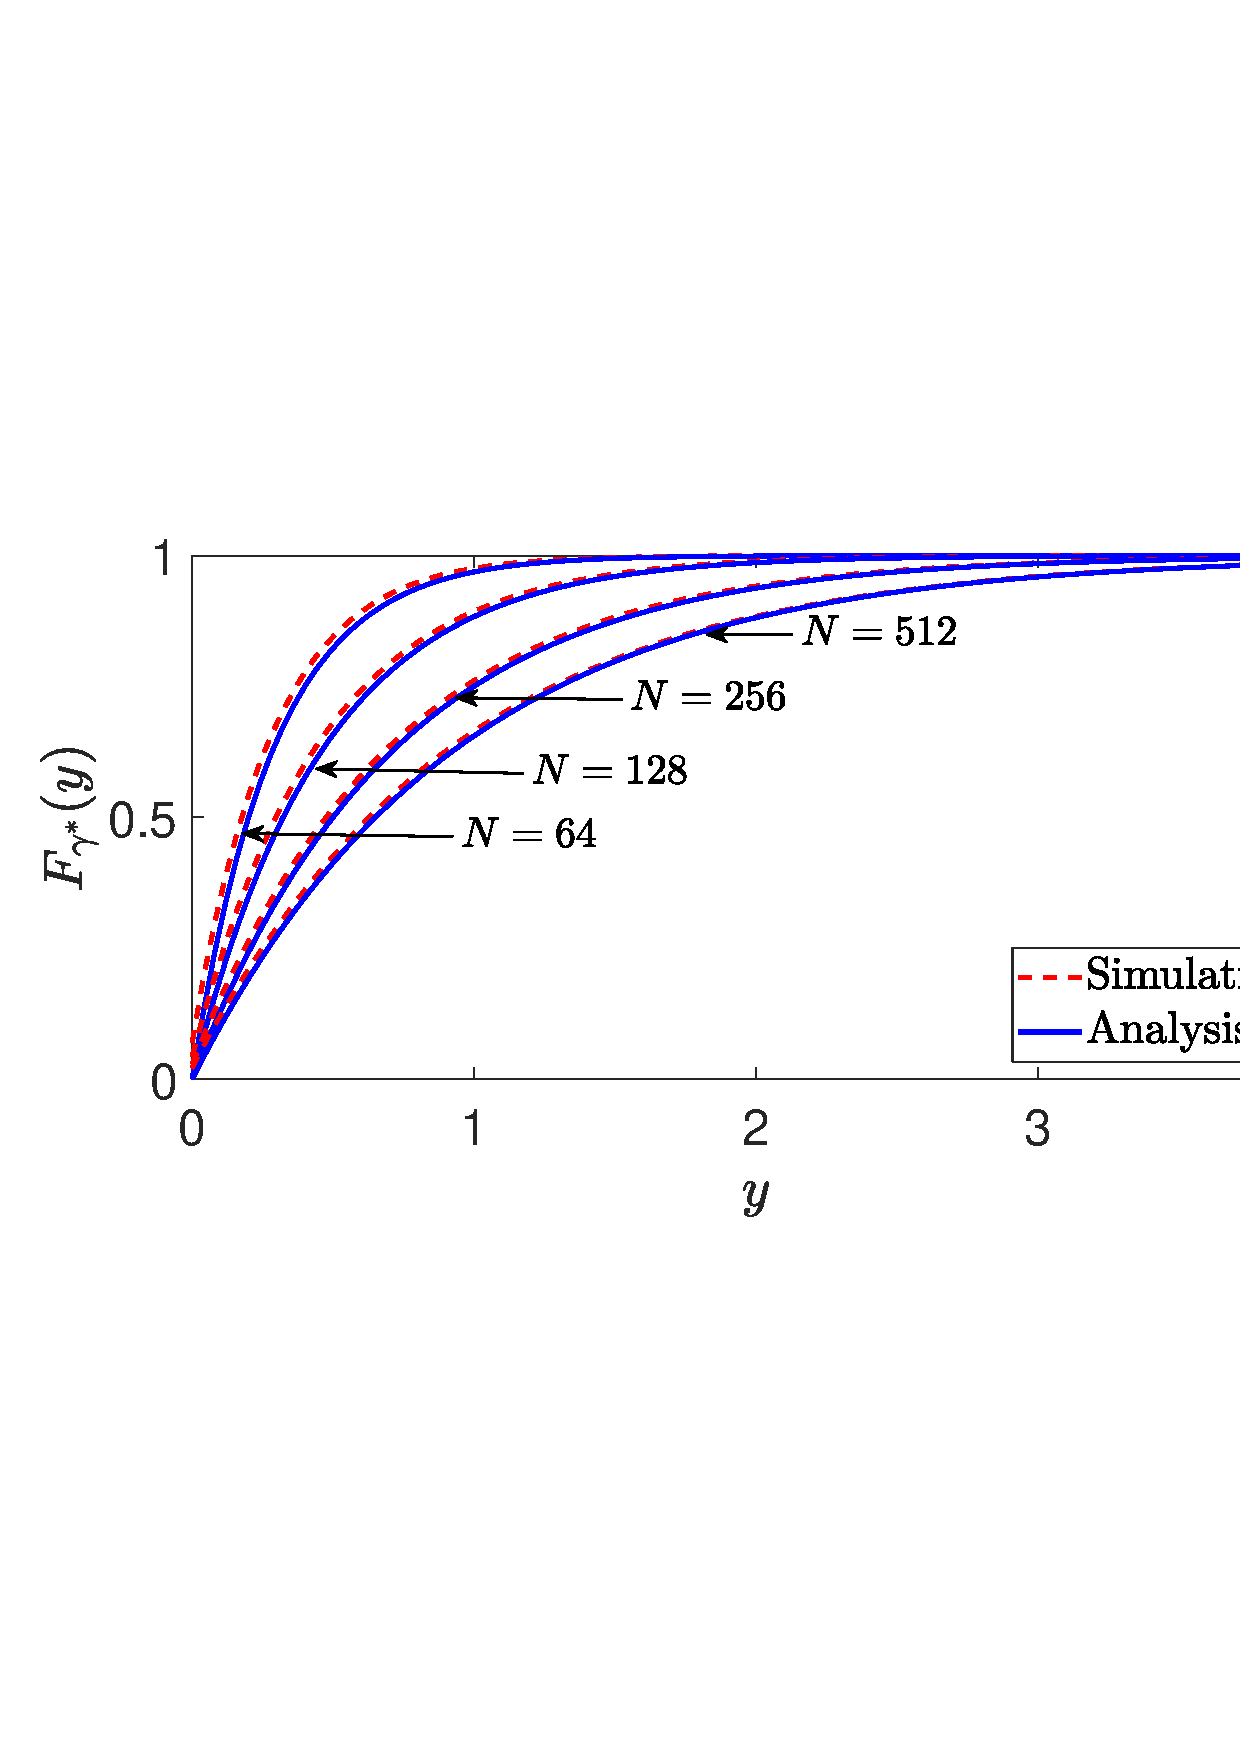
\includegraphics[width=5.6cm]{CDF_L_64_128_256_512_half.pdf}\label{fig:PDF_CDF_M_N}\vspace{-20mm}
			\caption{The CDF of  SNR ($\gamma^*$) for $N \in \{64, 128, 256, 512\}$ and $\bar{\gamma}= 10$ dB.}
		\end{figure}
		
	\end{minipage}\hspace{0.0cm}
	\begin{minipage}[t]{0.5\linewidth}	
		\begin{block}{}
			 Figure  illustrates that our analytical CDF approximation is accurate   for medium-to-large  numbers of reflective elements $(N)$ at the IRS.  A relatively larger $N$ is practically feasible and cost effective for IRSs, and hence, our probabilistic characterization of the optimal SNR  is useful in deriving performance bounds for the cascaded IRS-relay channels.  
		\end{block}
		
		 
		
	\end{minipage}
	
\end{frame}
%=====================================================================================
%=====================================================================================
\begin{frame}
\frametitle{Average Achievable Rate}
\begin{itemize}	
	\item The average achievable rate of the proposed system
	\begin{eqnarray}\label{eqn:avg_rate}
	\mathcal{R} = \E{\frac{1}{2}\log[2]{1+\gamma^*}}, \nonumber
	\end{eqnarray}   
	where the pre-log factor of $1/2$ is due to the fact that half-duplex relay mode requires two time-slots for end-to-end data transmission for the proposed system model.
	
	\item The exact derivation of  $\mathcal{R}$ seems mathematically intractable, and hence,  a  tight upper bound by invoking the Jensen’s inequality 
	\begin{eqnarray}\label{eqn:rate_up_bound}
	\mathcal{R} \leq \mathcal{R}_{ub} = \frac{1}{2}\log[2]{1+ \E{\gamma^*}}\approx \frac{1}{2}\log[2]{1+ \E{\tilde {\gamma}^*}}. \nonumber
	\end{eqnarray} 
	
	
	
	\item The closed-form expressions of  $\mathcal{R}_{ub}$
	\begin{eqnarray}\label{eqn:rate_up_bound_ana}
	\!\!\!\!\!\!\!\!\!\!\mathcal{R}_{ub} =\frac{1}{2}\log[2]{1+ 2 \psi \sigma_D^2 \mathcal{Q}\left(-\mu_R/\sigma_{R}\right) }. \nonumber
	\end{eqnarray} 
\end{itemize}

\end{frame}
%=====================================================================================
%=====================================================================================
\begin{frame}
\frametitle{The SNR/rate outage probability}
\begin{itemize}
	\item For the proposed system, the probability that the instantaneous SNR ($\gamma$) falls below a threshold SNR ($\gamma_{th}$) is referred as  the SNR outage probability.

	\item An approximation to this SNR outage probability 
	\begin{eqnarray}\label{eqn:out_prob}
	P_{out} = \mathrm{Pr}\left(\gamma^* \leq \gamma_{th}\right) \approx F_{\gamma^*}(\gamma_{th}). \nonumber
	\end{eqnarray}  
	
	\item The rate outage probability can also be readily obtained as
	\begin{eqnarray}
	P_{out} &=& \mathrm{Pr}\left(\mathcal{R}' \leq \mathcal{R}_{th}\right) = \mathrm{Pr}\left(\gamma^* \leq 2^{2\mathcal{R}_{th}}-1\right) \nonumber \\
	&\approx& F_{\gamma^*}(2^{2\mathcal{R}_{th}}-1),\nonumber
	\end{eqnarray}
	where $\mathcal{R}'=\frac{1}{2}\log[2]{1+\gamma^*}$ is the achievable rate, and $\mathcal{R}_{th}$ denotes a threshold rate. 
	
\end{itemize}

\end{frame}
%=====================================================================================
%=====================================================================================
\begin{frame}
\frametitle{The average symbol error rate (SER)}
\begin{itemize}
	\item The average SER of the proposed systems is defined as the expectation of  conditional error probability $(P_{e|\gamma^*})$ over the  probability distribution of $\gamma^*$.
	
	\item  $P_{e|\gamma^*}$ is given for a broad range of coherent modulation schemes by $P_{e|\gamma^*} = \omega \mathcal{Q}\left(\sqrt{\vartheta \gamma^*}\right)$, where the modulation scheme determines the values of fixed  parameters $\omega$ and $\vartheta$.
	
	\item Thus, the average SER:  $\bar{P}_e= \E{\omega \mathcal{Q}\left(\sqrt{\vartheta \gamma^*}\right)}$.
	
	\item A tight approximation for $\bar{P}_e$ can be given as 
	\begin{eqnarray}\label{eqn:ser_cdf}
	\bar{P}_e \approx \frac{\omega}{2} - \frac{\omega \sqrt{\vartheta}}{2 \sqrt{2 \pi}} \int_{0}^{\infty} x^{-1/2} \Exp{-\frac{\vartheta x}{2}} \bar{F}_{\tilde{\gamma}^*}(x) dx, \nonumber
	\end{eqnarray} 
	where $\bar{F}_{\tilde{\gamma}^*}(x)=1-F_{\tilde{\gamma}^*}(x)$ is the CCDF of $\gamma^*$.
	
	\item The closed-form solution to $\bar{P}_e $ 
	\begin{eqnarray}\label{eqn:ser_ana}
	\!\!\!\!\!\bar{P}_e \!&\approx&\! \frac{\omega}{2} \!+\! 2\lambda \mathcal{Q}\left(-\mu_R/\sigma_{R}\right) \!+\! \frac{\lambda}{\pi \sqrt{a \sigma_{R}^2}} \exp{\frac{-\mu_R^2}{2\sigma_{R}^2}\left(1-\frac{1}{2a\rho \sigma_{R}^2}\right)} \nonumber \\
	&&\!\!\!\!\!\!\!\!\! \times \! \sum\nolimits_{i \in C_{\infty}} (-2)^i \left(\frac{\sqrt{a} \rho^2 \sigma_{R}^2}{\mu_R}\right)^{i+1} \Gamma\left(\frac{i+1}{2}, \frac{\mu_R^2}{2a\rho \sigma_{R}^4}\right). \nonumber
	\end{eqnarray}
	
\end{itemize}

\end{frame}
%=====================================================================================
%=====================================================================================
\begin{frame}
	\frametitle{Effects of Phase Quantization}
	\begin{itemize}	
		\item In practice, an IRS reflecting element  only uses  a set of discrete phase-shifts due to the associated hardware limitations.
		
		\item We investigate the impact of phase-shift quantization assuming that a limited number of discrete phase-shift is available for selection at the $n$th IRS element as 
		$\hat{\theta}_n^* = \pi \hat{q}/2^{b-1}$,
		\begin{itemize}
			\item[$\circ$] $b$ is the number of quantization bits
			\item[$\circ$] $\hat{q} = \underset{q \in \{0, \pm 1, \cdots, \pm 2^{b-1}\}}{ \mathrm{argmin}} \;{|\theta_n^* - \pi q/2^{b-1}|}$
			\item[$\circ$] $\hat{\theta}_n^*$ is the optimal phase-shift
		\end{itemize}
		
		\item The difference between unquantized and quantized phase-shift is defined as the phase quantization error:	$\epsilon_n = \theta_n^* - \hat{\theta}_n^*$.
		
		\item When the number of quantization levels increases, $\epsilon_n$ converges to a uniform distribution as $ \epsilon_n \sim \mathcal{U} [-\pi/2^b, \pi/2^b)$.
		
		\item The optimal SNR  with discrete phase-shift
		\begin{eqnarray} \label{eqn:opt_SNR}
		\hat{\gamma}^*=\frac{\bar{\gamma}_R \bar{\gamma}_D   \beta_{h^D}^2  \left(\sum_{n \in \mathcal{N}} \eta_{n} \beta_{h_{n}^R}  \beta_{h_{n}^I} \exp{j\epsilon_n}\right)^2}{ \bar{\gamma}_R \left(\sum_{n \in \mathcal{N}} \eta_{n} \beta_{h_{n}^R}  \beta_{h_{n}^I} \exp{j\epsilon_n} \right)^2  + \bar{\gamma}_D \beta_{h^D}^2 +1 }. \nonumber
		\end{eqnarray}
	

	\end{itemize}
	
\end{frame}
%=====================================================================================
%=====================================================================================
\begin{frame}
	\frametitle{Simulation: Outage probability}
	\vspace{-2.6mm}
\begin{figure}
\centering
\includegraphics[width=8cm]{outage_L_64_128_256_512_without}\vspace{-3mm}
\caption{The outage probability for $N \in \{64,128,256,512\}$ and the threshold SNR is  $\gamma_{th}=0$ dB. .}
\label{fig:outage_L_64_128_256_512_without}
\end{figure}
\end{frame}
%=====================================================================================
%=====================================================================================
\begin{frame}
	\frametitle{Simulation: Average achievable rate}
	\vspace{-2.6mm}
	\begin{figure}
		\centering
		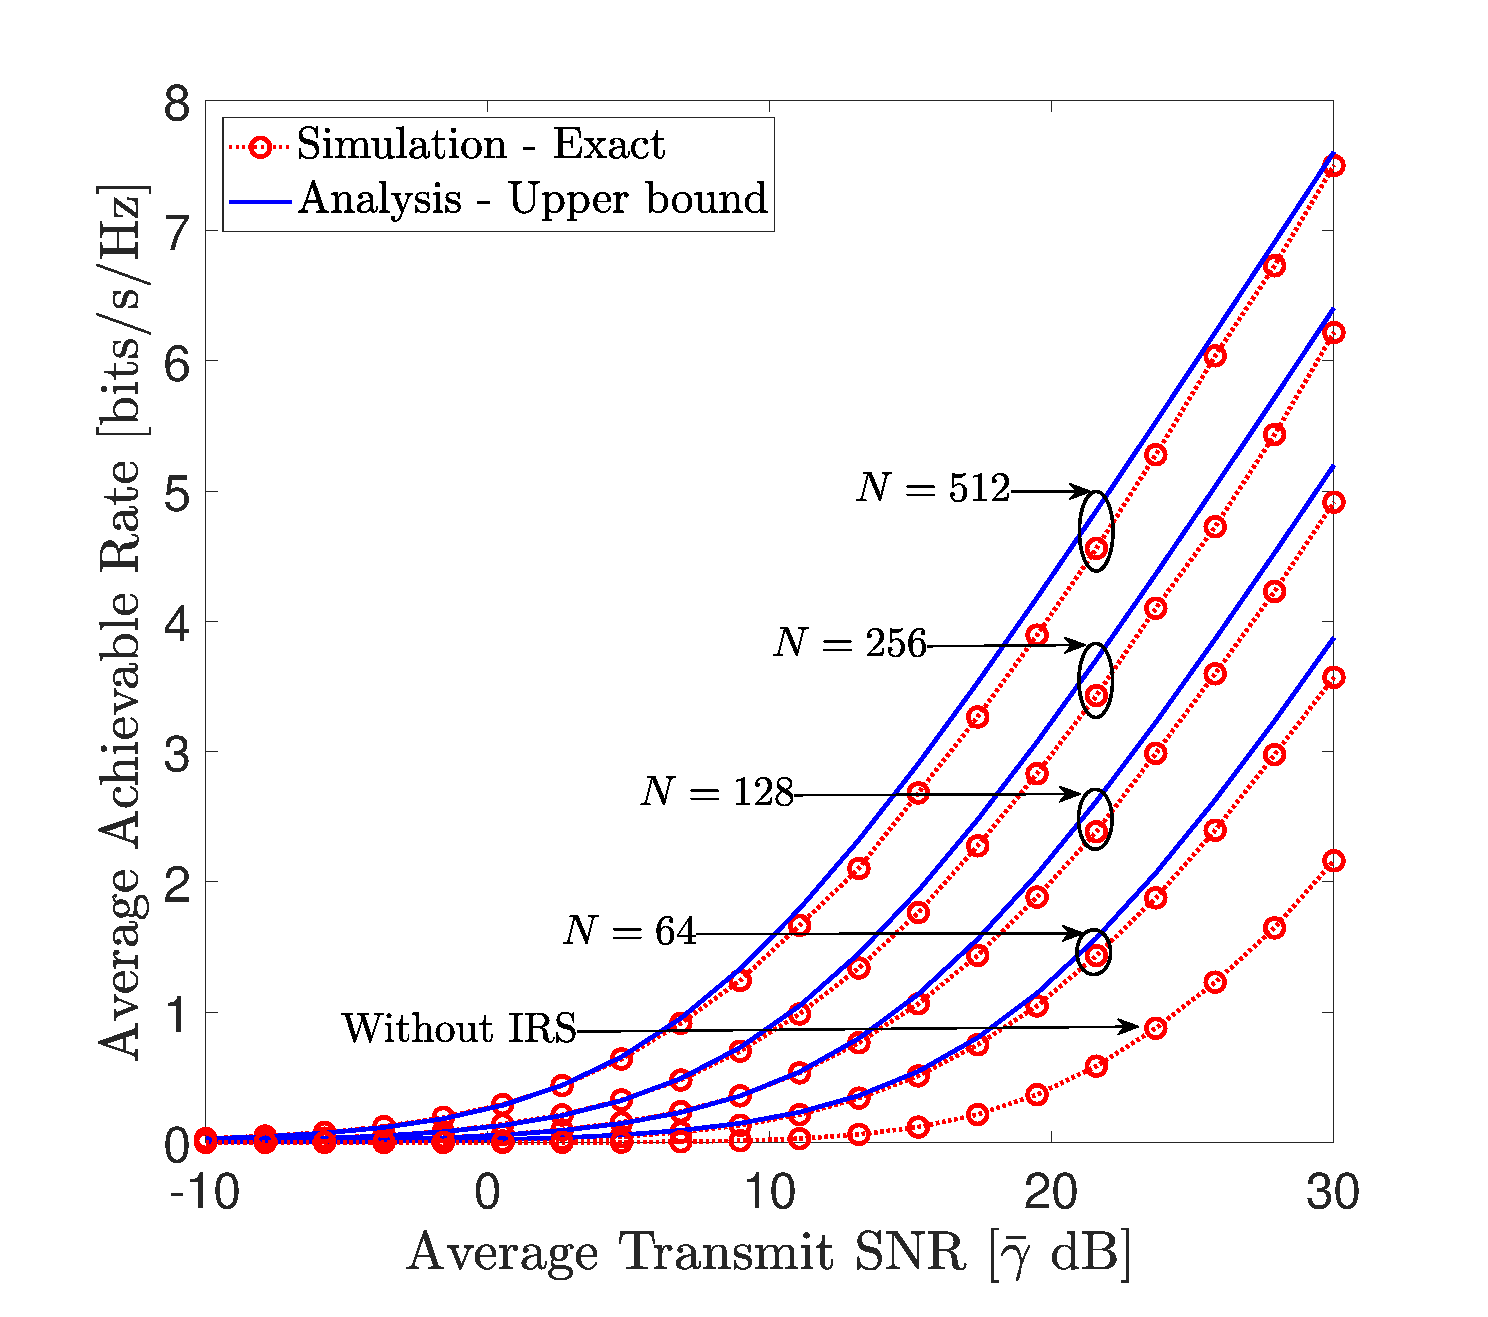
\includegraphics[width=8cm]{rate_L_64_128_256_512_without}\vspace{-3mm}
		\caption{The average achievable rate for $N \in \{64,128,256,512\}$.}
		\label{fig:rate_L_64_128_256_512_without}
	\end{figure}
\end{frame}
%=====================================================================================
%=====================================================================================
\begin{frame}
\frametitle{Simulation: Average BER}
\vspace{-2.6mm}
\begin{figure}
	\centering
	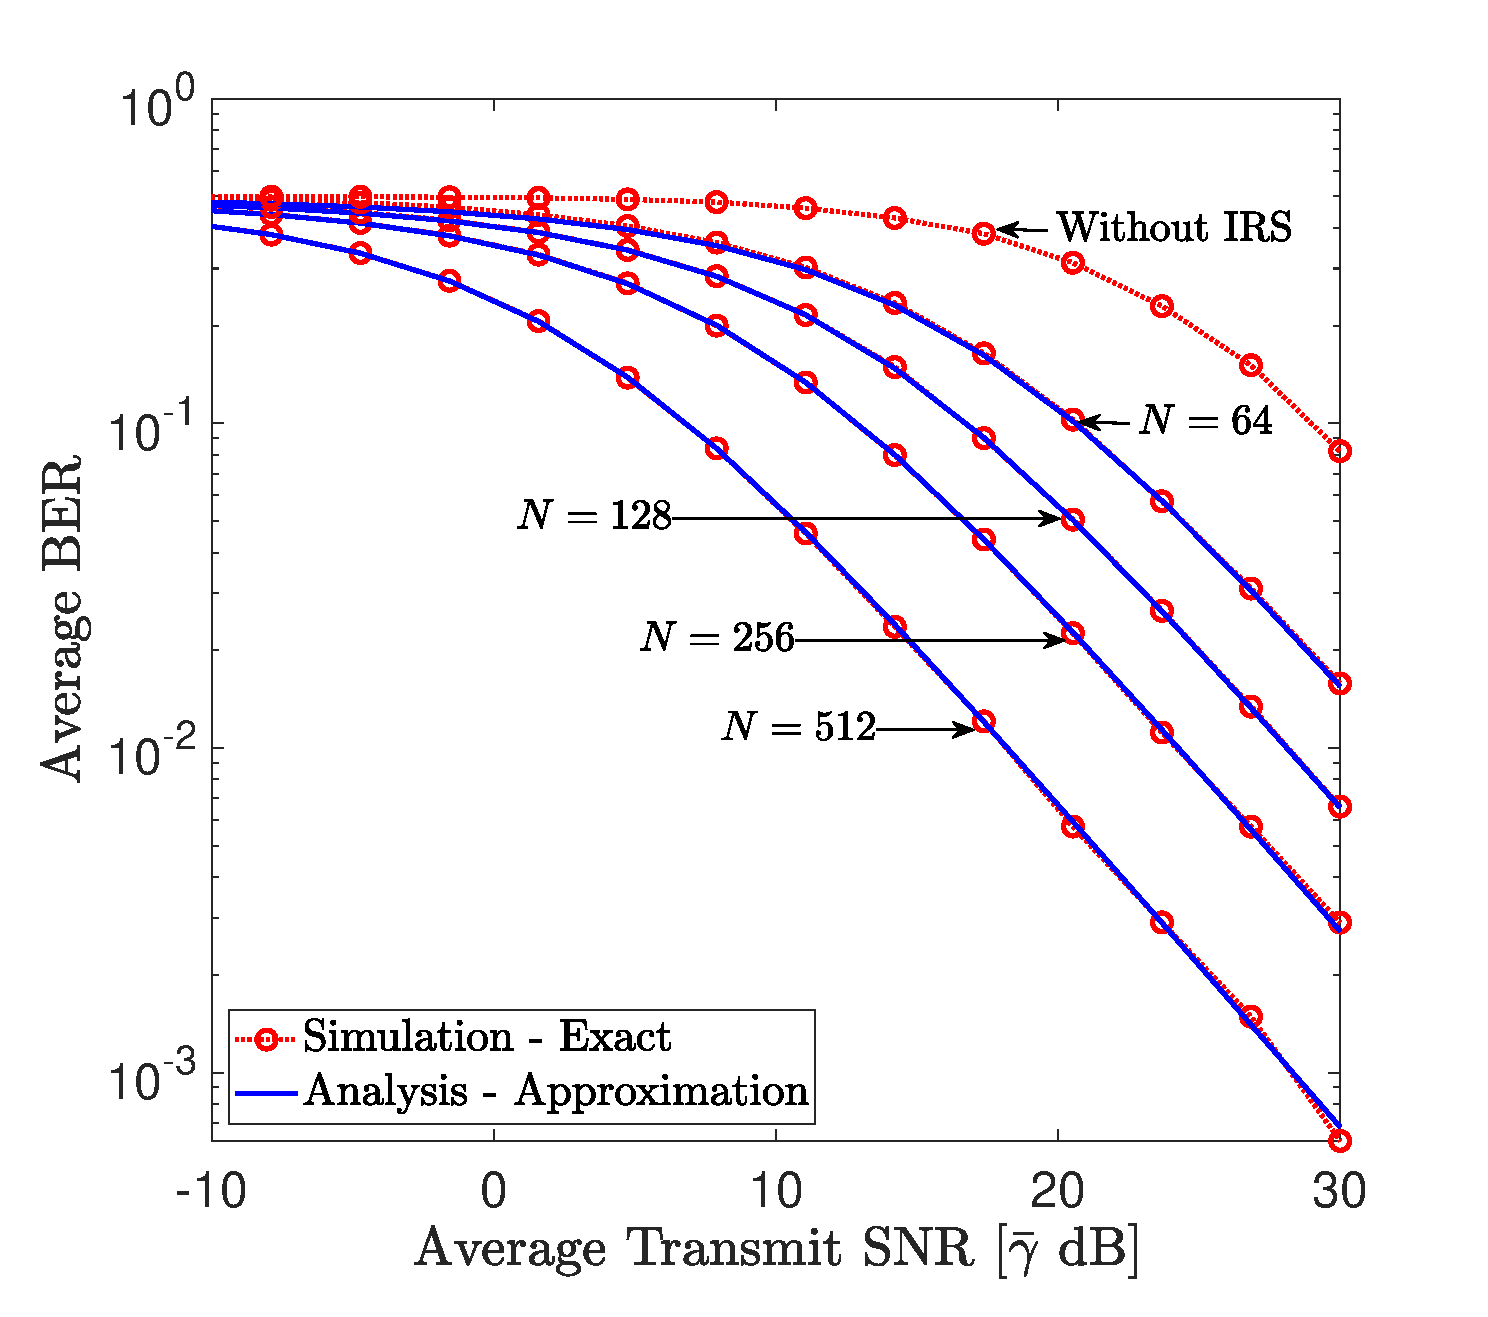
\includegraphics[width=8cm]{ber_L_64_128_256_512_without}\vspace{-3mm}
	\caption{The average BER of BPSK for $N \in \{64,128,256,512\}$, $\omega=1$, and $\vartheta=2$.}
	\label{fig:ber_L_64_128_256_512_without}
\end{figure}
\end{frame}
%=====================================================================================
%=====================================================================================
\begin{frame}
	\frametitle{Simulation: Phase-shift quantization}
	\vspace{-2.6mm}
	\begin{figure}
		\centering
		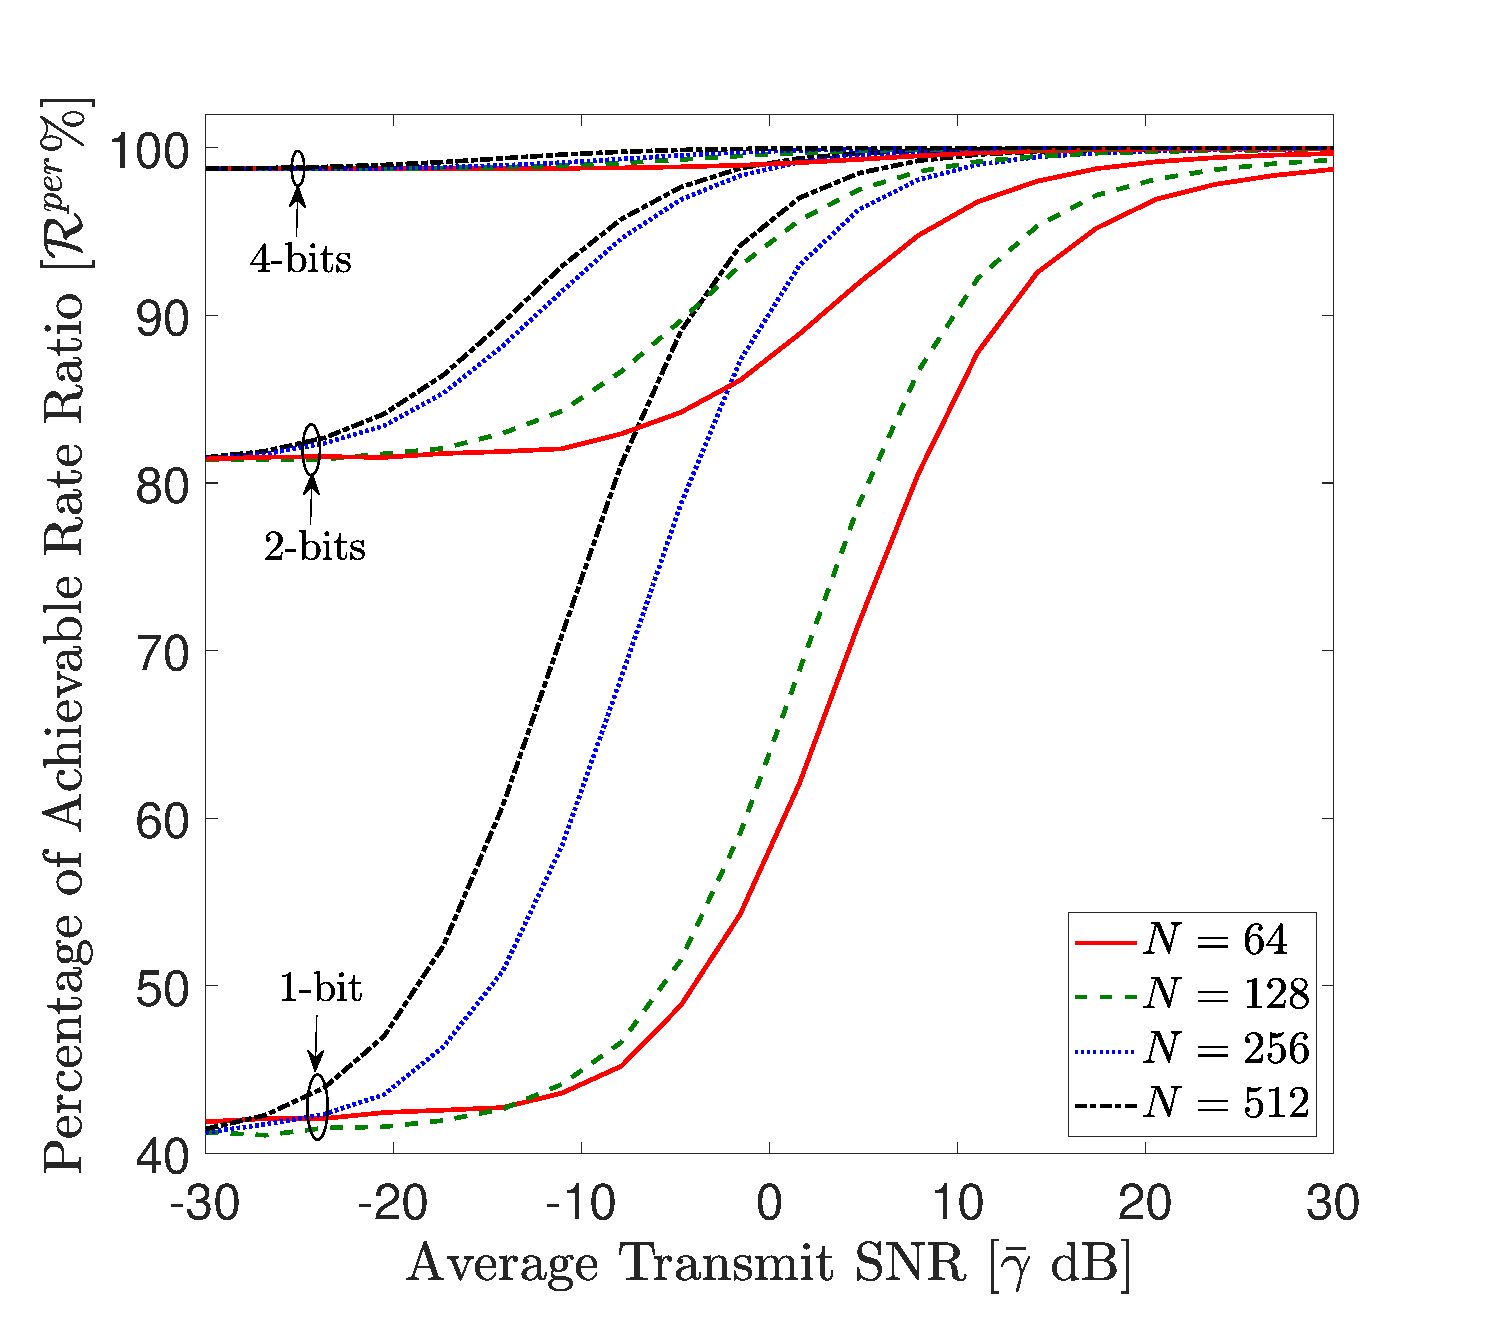
\includegraphics[width=8cm]{Rate_gain_q}\vspace{-3mm}
		\caption{The effect of phase shift quantization on the average achievable rate for $N \in \{64,128,256,512\}$.}
		\label{fig:Rate_gain_q}
	\end{figure}
\end{frame}
%=====================================================================================
%=====================================================================================
\begin{frame}
	\frametitle{Conclusions}
	\begin{itemize}
		\item The performance  of an IRS-assisted relay system has been investigated.
		
		\pause
		\item The optimal SNR  that is attained through   intelligent phase-shift controlling of the IRS elements has been probabilistically characterized   by deriving a tight CDF  approximation.
		
		\pause
		\item Thereby, tight approximations/bounds for the  fundamental performance metrics, including the average achievable rate, SNR/rate outage probability,  and  average SER have been derived.
		
		\pause
		\item The impact of phase-shift errors at the IRS has been investigated by adopting discrete phase-shift adjustments.
		
		\pause
		\item The accuracy of our analysis has been validated through the Monte-Carlo simulation.
		
		\pause
		\item A rigorous set of numerical results has been presented to investigate the performance of the proposed IRS-assisted relay system.
		
		\pause
		\item From our numerical results, we  reveal that the IRS-assisted relay systems can  enhance the end-to-end wireless communication performance.
		
	\end{itemize}


\end{frame}
%=====================================================================================
%=====================================================================================
\begin{frame}
\frametitle{References}
\begin{enumerate}
	\item {\color{TUM_blau} HC. Liaskos et al., “{A New Wireless Communication Paradigm Through
		Software-Controlled Metasurfaces},” {in} IEEE Commun. Mag., vol. 56, no. 9,
		pp. 162–169, 2018.}
	
	\item {\color{TUM_blau} D. L. Galappaththige, D. Kudathanthirige, and G. Amarasuriya Aruma
		Baduge, “{Performance Analysis of Distributed Intelligent Reflective Surface
		Aided Communications},” {in} IEEE Global Commun. Conf. (GLOBECOM),
		May 2020, pp. 1–6,.}
		
	\item {\color{TUM_blau} G. Amarasuriya, C. Tellambura, and M. Ardakani, “{Asymptotically-Exact
		Performance Bounds of AF Multi-Hop Relaying over Nakagami Fading},” {in}
		IEEE Trans. Commun., vol. 59, no. 4, pp. 962–967, 2011.}
		
	\item {\color{TUM_blau} E. Bj{\"o}rnson, {\"O} . {\"O} zdogan, and E. G. Larsson, “{Intelligent Reflecting
		Surface Versus Decode-and-Forward: How Large Surfaces are Needed
		to Beat Relaying?}”, {in} IEEE Wireless Commun. Lett., vol. 9, no. 2, pp. 244–
		248, 2020.}
		
	\item {\color{TUM_blau} M. Di Renzo et al., “{Reconfigurable Intelligent Surfaces vs. Relaying:
		Differences, Similarities, and Performance Comparison},” {in} IEEE Open J.
		Commun. Society, vol. 1, pp. 798–807, 2020.}
	
\end{enumerate}



\end{frame}
%=====================================================================================
%=====================================================================================
\begin{frame}
		\begin{center}
		\LARGE \bf Thank you for your attention!
	\end{center}
		\begin{center}
	\bf Questions ?? 
	
	{\color{blue} alan.devkota@siu.edu}
	
	{\color{blue} diluka.lg@siu.edu}
	
\end{center}
\end{frame}
%=====================================================================================



%
%}% --------------------------------------------------------
%
%
%% ========================================
%\bibliographystyle{IEEEtran}



\end{document}